\documentclass[10pt]{beamer}

%%%
% PREAMBLE FOR THIS DOC 
%%%
%https://tex.stackexchange.com/questions/68821/is-it-possible-to-create-a-latex-preamble-header
\usepackage{/Users/miw267/Repos/csci246_spring2025/slides/preambles/beamer_preamble_for_CSCI246}



%%% TRY TO RESHOW TOC AT EACH SECTION START (with current section highlighted)
% Reference: https://tex.stackexchange.com/questions/280436/how-to-highlight-a-specific-section-in-beamer-toc
\newcommand\tocforsect[2]{%
  \begingroup
  \edef\safesection{\thesection}
  \setcounter{section}{#1}
  \tableofcontents[#2,currentsection]
  \setcounter{section}{\safesection}
  \endgroup
}


%%%% HERES HOW TO DO IT CORRECTLY
% FIRST IN .STY FILE, DO
%\usetheme[sectionpage=none]{metropolis}
% THEN AT EACH SECTION DO
%\begin{frame}{Outline}
%  \tableofcontents[currentsection]	
%\end{frame}



%\setbeamertemplate{navigation symbols}{}
%\setbeamertemplate{footline}[frame number]{}


%%%
% DOCUMENT
%%%

\begin{document}

%\maketitle

%% Title page frame
%\begin{frame}
%    \titlepage 
%\end{frame}





\title{02/03/2025: More Induction}
\author{CSCI 246: Discrete Structures}
\date{Textbook reference: Ch. 4, Hampkins}

\begin{frame}
    \titlepage 
\end{frame}


\begin{frame}
\footnotesize 

\begin{mygreenbox}[title=Graded Quiz Pickup]
Quizzes are in the front of the room, grouped into four bins (A-G, H-L, M-R, S-Z) by last name. The quizzes are upside down with your last name on the back. Come find yours before, during, or after class.  Only turn the quiz over if it's yours.
\end{mygreenbox} 
\vfill 

\begin{myredbox}[title=Review of Make Up Policy / Grading Policy]

\begin{itemize}
\item No makeup quizzes for absences.  But 3 reading quizzes / 3 participations / 1 problems quiz are dropped.  
\item What about protection against occasionally getting a low quiz score? As of last week, I am sprinkling in extra credit to some quizzes.   
\end{itemize}

\end{myredbox}

\vfill 


\begin{myyellowbox}[title=Today's Agenda]
\begin{itemize}
	\item Reading \& problems quizzes  (5 mins)
	\item Mini-lecture ($\approx$ 15 mins)
	%
	\begin{itemize}
	\footnotesize 
	\item Review Boolean Algebra
	\item Induction 
	\end{itemize}
	%
	\item Group exercises ($\approx$ 30 mins)
\end{itemize}

\end{myyellowbox}
\vfill 

\end{frame}




\begin{frame}{Today's Quiz}

\begin{myyellowbox}[title=Logistics Alert]
Please write your last name on the back of the page. 
\end{myyellowbox}

\vfill


 \begin{mygreenbox}[title=Reading Quiz (Induction)]
Prove that every positive integer has a prime factorization (i.e. can be expressed as the product of prime numbers).
\end{mygreenbox}

\vfill 

\begin{myredbox}[title=Bonus Alert]
This quiz is extra credit.
\end{myredbox}


\end{frame}



\begin{frame}{Problems Quiz Scores: Proofs and Counterexamples}

\begin{figure}[ht]
        \centering
        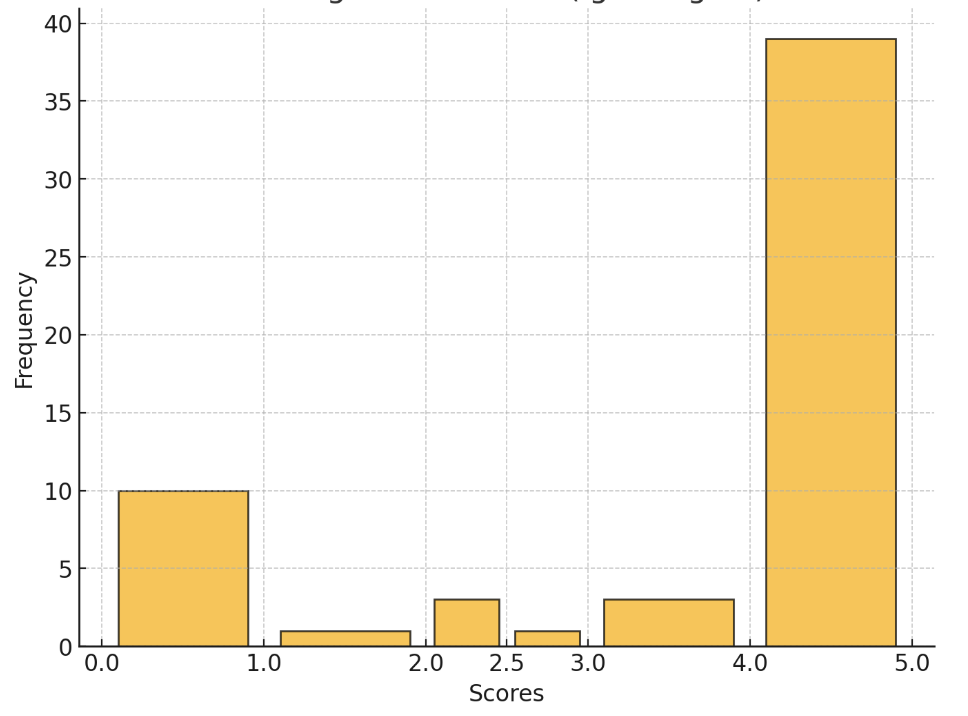
\includegraphics[width=.8\textwidth]{images/problems_quiz_scores}
        \caption{Median Score = 5.0 / 5.0}
\end{figure}
\vfill 

\end{frame}


\begin{frame}{Reading Quiz Scores: Induction}

\begin{figure}[ht]
        \centering
        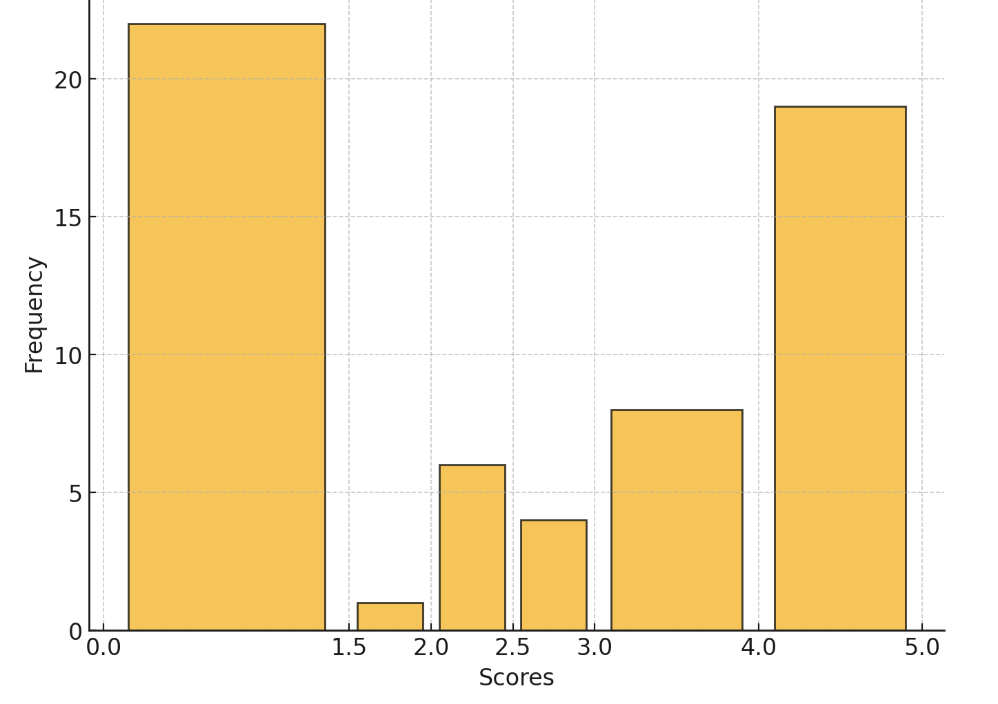
\includegraphics[width=.8\textwidth]{images/ch4_reading_quiz_scores}
   		\caption{Median Score = 2.5 / 5.0}
\end{figure}
\vfill 

\end{frame}

\begin{frame}[standout]
Review Boolean Algebra Group Exercises.
	
\end{frame}

\begin{frame}{Strong Induction}
\footnotesize
 \begin{mygreenbox}[title=Strong Induction]
Assume that $A$ is a set of natural numbers with the property that, for every natural number $n$, if every number smaller than $n$ is in $A$, then $n$ itself is in $A$. Then every natural number is in $A$.
\end{mygreenbox}

\vfill 

 \begin{myredbox}[title=When to Use Strong Induction]
 Sometimes there are scenarios where the induction implication goes naturally not from $n$ to $n+1$, but:
 \begin{itemize}
 \item From some smaller number to $n+1$, or
 \item From several smaller numbers	
 \end{itemize}
 \end{myredbox}

\vfill 
 \begin{myyellowbox}[title=Example: Every positive integer has a prime factorization]
 \begin{itemize}
 \item Suppose every number smaller than $n$ has a prime factorization.
 \item The number $n$ must either be prime (in which case we are done) or composite.
 \item If $n$ is composite, then $n=ab$ for smaller number $a,b<n$.  But $a,b$ have their own  factorizations by the induction hypothesis.  These can be put together to make a prime factorization of $n$.
 \end{itemize}

 \end{myyellowbox}
\end{frame}





\begin{frame}
\footnotesize
Group 1: aaron.loomis,lucas.jones6,jonas.zeiler\\
Group 2: sarah.periolat,mason.barnocky,emmeri.grooms\\
Group 3: nolan.scott1,jack.fry,connor.mizner\\
Group 4: adam.wyszynski,julia.larsen,carsten.brooks\\
Group 5: peter.buckley1,jacob.ruiz1,colter.huber\\
Group 6: alexander.knutson,conner.reed1,pendleton.johnston\\
Group 7: michael.oswald,evan.schoening,joseph.triem\\
Group 8: samuel.hemmen,connor.yetter,anthony.mann\\
Group 9: lynsey.read,owen.obrien,jakob.kominsky\\
Group 10: cameron.wittrock,connor.graville,tyler.broesel\\
Group 11: delaney.rubb,jett.girard,evan.barth\\
Group 12: derek.price4,alexander.goetz,ryan.barrett2\\
Group 13: zeke.baumann,griffin.short,william.elder1\\
Group 14: jada.zorn,matthew.nagel,ethan.johnson18\\
Group 15: jacob.ketola,luke.donaldson1,yebin.wallace\\
Group 16: jeremiah.mackey,jacob.shepherd1,erik.moore3\\
Group 17: justice.mosso,carver.wambold,samuel.rollins\\
Group 18: joseph.mergenthaler,james.brubaker,john.fotheringham\\
Group 19: micaylyn.parker,devon.maurer,reid.pickert\\
Group 20: timothy.true,caitlin.hermanson,kaden.price\\
Group 21: peyton.trigg,samuel.mosier,blake.leone\\
Group 22: tristan.nogacki,bridger.voss,luka.derry\\\end{frame}


\begin{frame}{Group exercises: Induction}
\footnotesize 

\begin{enumerate}
\item Show by induction that $n^2-n$ is even for any natural number $n$ (that is, for $n=0,1,2,\hdots$).
\item  Show by induction that $2^n < n!$ for all $n \geq 4$.	
\item Show by induction that $f_0 + \cdots + f_n = f_{n+2} -1$ in the Fibonacci sequence.
\item Show by induction that $f_n < 2^n$ in the Fibonacci sequence. 
\end{enumerate}
\vfill 
\begin{mygreenbox}[title=Definition]
The \textbf{Fibonacci sequence} is the sequence given by the following recursive rules:
\[f_0 =0, \qquad \quad f_1 =1, \qquad \quad f_{n+2} = f_n + f_{n+1} \]
The sequence is: $0,1,1,2,3,5,8,13,21,34, \hdots$
\end{mygreenbox}
\vfill 
\begin{myyellowbox}[title=Logistics Alert]
 \#1 has been carried over from Friday.	
\end{myyellowbox}

\end{frame}

\begin{frame}[standout]
Solutions to group exercises.	
\end{frame}


\begin{frame}
\small 
\begin{mygreenbox}[title=Exercise 1]
Show by induction that $n^2-n$ is even for any natural number $n$ (that is, for $n=0,1,2,\hdots$).
\end{mygreenbox}

\vfill \vfill 
\begin{myyellowbox}[title=Solution]
\textbf{Induction base.} Take $n=0$.  Then $n^2-n = 0^2-0 = 0$, which is even. So $n^2-n$ is even when $n=0$.

\vspace{0.5cm}

\textbf{Induction step.} Now we \underline{assume} the proposition holds at index $n$ (this is called the \alert{induction hypothesis}), and we \underline{need to show} it holds at index $n+1$.  That is, we assume $n^2-n$ is even, and we need to show that $(n+1)^2-(n+1)$ is even.  We have
%
\begin{align*}
(n+1)^2-(n+1) &= (n^2+2n+1) - (n+1) \\
&= n^2+n  \\
&= \explaintermbrace{even by induct. hypoth.}{(n^2 -n)} \; + \; \explaintermbrace{even by def. even}{(2n)}  && \scripttext{(subtract, add $n$)}	
\end{align*}
And the sum of two even numbers is even.

Hence, $n^2-n$ is even $\implies (n+1)^2-(n+1)$ is even.
\end{myyellowbox}

\end{frame}

\begin{frame}
\begin{mygreenbox}[title=Exercise 2]
 Show by induction that $2^n < n!$ for all $n \geq 4$.	
\end{mygreenbox}

\vfill \vfill 
\begin{myyellowbox}[title=Solution]
\textbf{Induction base.} Take $n=4$.  Then $2^n = 2^4 = 16$ and $n! = 4! = 4 \cdot 3 \cdot 2 \cdot 1 = 24$. So $2^n < n!$ when $n=4$.

\vspace{0.5cm}

\textbf{Induction step.} Now we \underline{assume} $2^n<n!$ (this is called the \alert{induction hypothesis}), and we \underline{need to show} $2^{n+1}<(n+1)!$ We have
%
\begin{align*}
2^{n+1} &= 2 \cdot 2^n \\
&< 2 \cdot n! && \scripttext{(by the induction hypothesis)} \\
&< (n+1) \cdot n! && \scripttext{(since $n \geq 4$)} \\
&= (n+1)! && \scripttext{(by def. factorial)}	
\end{align*}
Hence, $2^n<n! \implies 2^{n+1}<(n+1)!$
\end{myyellowbox}
\end{frame}




\begin{frame}

\begin{mygreenbox}[title=Exercise 3]
Show by induction that $f_0 + \cdots + f_n = f_{n+2} -1$ in the Fibonacci sequence.	
\end{mygreenbox}

\vfill \vfill 
\begin{myyellowbox}[title=Solution]
\textbf{Induction base.} Take $n=0$.  Then $f_0 + \cdots + f_n = f_0 =0$ and $f_{n+2} -1 = f_2 -1 = 1-1 = 0$. So $f_0 + \cdots + f_n = f_{n+2} -1$ when $n=0$.

\vspace{0.25cm}

\textbf{Induction step.} Now we \underline{assume} the proposition holds at index $n$ (this is called the \alert{induction hypothesis}), and we \underline{need to show} it holds at index $n+1$.  That is, we assume $f_0 + \cdots + f_n = f_{n+2} -1$, and we need to show that $f_0 + \cdots + f_{n+1} = f_{n+3} -1$.  We have
%
\begin{align*}
f_0 + \cdots + f_{n+1} &= (f_0 + \cdots + f_n) + f_{n+1} \\
&=(f_{n+2} -1) + f_{n+1} && \scripttext{(by the induction hypothesis)} \\
&= (f_{n+1}+f_{n+2}) -1  && \\
&= f_{n+3} -1  && \scripttext{(by def. Fibonacci number)}	
\end{align*}
Hence, if the proposition holds at index $n$, it holds at index $n+1$.
\end{myyellowbox}
	
\end{frame}


\begin{frame}
\small 
\begin{mygreenbox}[title=Exercise 4]
Show by induction that $f_n < 2^n$ in the Fibonacci sequence. 
\end{mygreenbox}

\vfill \vfill 
\begin{myyellowbox}[title=Solution]
\textbf{Induction base.} Take $n=0$.  Then $f_n = f_0 = 0$  and  $2^n =2^0 =1$. So $f_n < 2^n$ when $n=0$.

\vspace{0.25cm}

\textbf{Induction step.} Here we use strong induction. We \underline{assume} the proposition holds at indices $1, 2, \hdots n$ (this is the \alert{(strong) induction hypothesis}), and we \underline{need to show} it holds at index $n+1$.  That is, we assume $f_k < 2^k$ for $k=1,\hdots, n$, and we need to show that $f_{n+1} < 2^{n+1}$.  We have
%
\begin{align*}
f_{n+1} &= f_n + f_{n-1} && \scripttext{(by def. Fibonacci number)}	\\
&< 2^n + 2^{n-1} && \scripttext{(by the (strong) induction hypothesis)} \\
&< 2^n + 2^n  && \\
&= 2 \cdot 2^n  \\
&= 2^{n+1}.
\end{align*}
Hence, $f_n < 2^n \implies f_{n+1} < 2^{n+1}$.
\end{myyellowbox}
	
\end{frame}

\end{document}
